% !TEX root = thesis.tex

%%
%%
%% Discussion chapter
%%
%%

We are investigating the effectiveness of the \gls{dkd} in estimating the incidence risk of chronic diseases. 
The \gls{dkd} is computed by taking a kernel estimate of the disease incidence intensity and dividing by a kernel estimate of the population density at any given point.
We ran several scenarios to examine how variations in the incidence risk function,
the population, and the sample size affect the accuracy of the estimation. 
We used several methods to measure the accuracy of the \gls{dkd} estimate,
as described in \Cref{sec:method:accuracy}.

As can be seen in \Cref{fig:discussion:overall_nmise_boxplot},
the \gls{nmise} for the \gls{oracle} selected bandwidth was, on average,
lower than for the other bandwidth selectors.
The \gls{cv} and \gls{silverman} selectors had similar performance.
All of these bandwidth selection techniques are optimized to minimize \gls{mise},
and so these results are what we expected.
The scale of the \gls{nmise} is much higher when the population is not uniform.
Although on average, the \gls{cv} and \gls{silverman} selectors have similar performance for the peaked populations,
the variance of the \gls{cv} selector is much higher.

\begin{figure}[htbp]
    \centering
    \begin{subfigure}[t]{0.45\textwidth}
        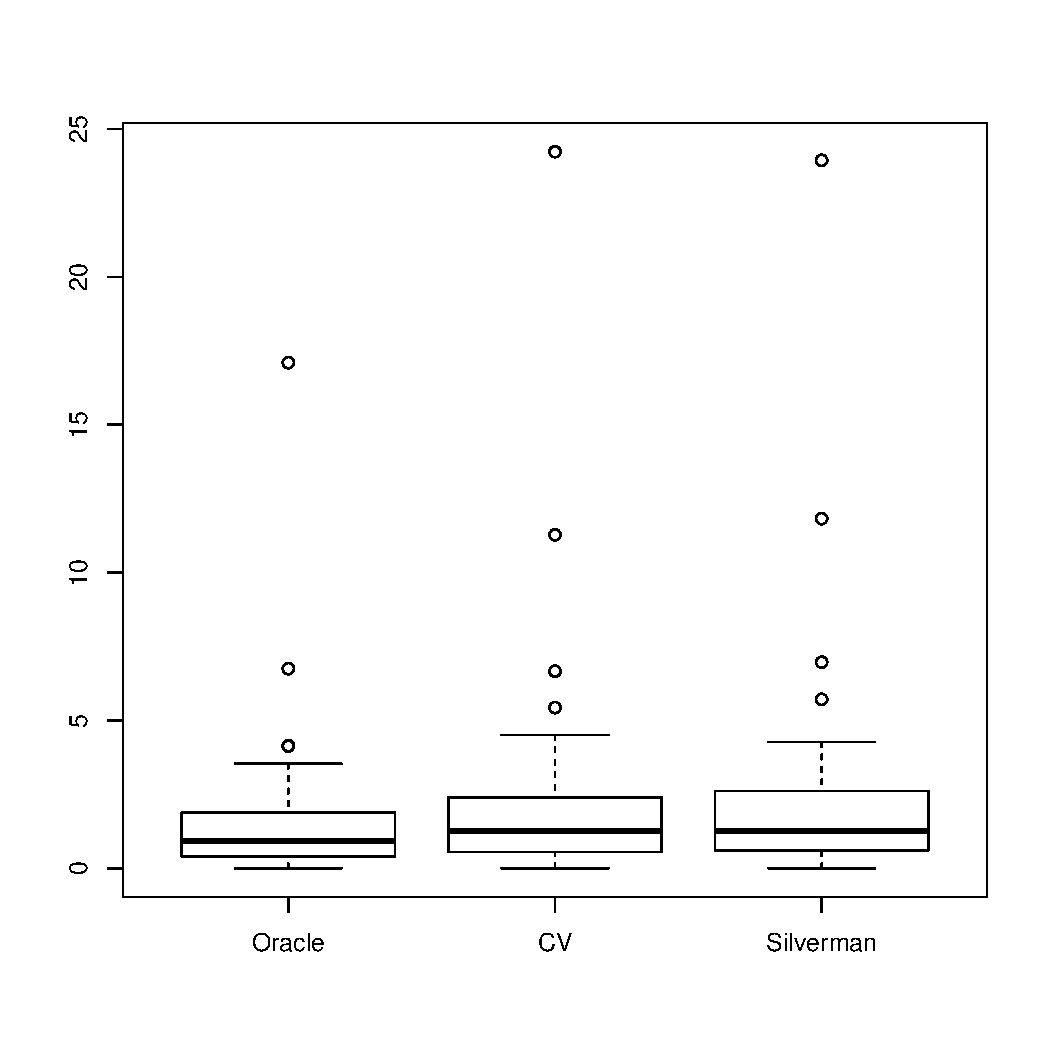
\includegraphics[width=\textwidth]{results/by_overall/normalized-mise-boxplot}
        \subcaption{Uniform populations}
        \label{fig:discussion:overall_nmise_boxplot:unif}
    \end{subfigure}
    \begin{subfigure}[t]{0.45\textwidth}
        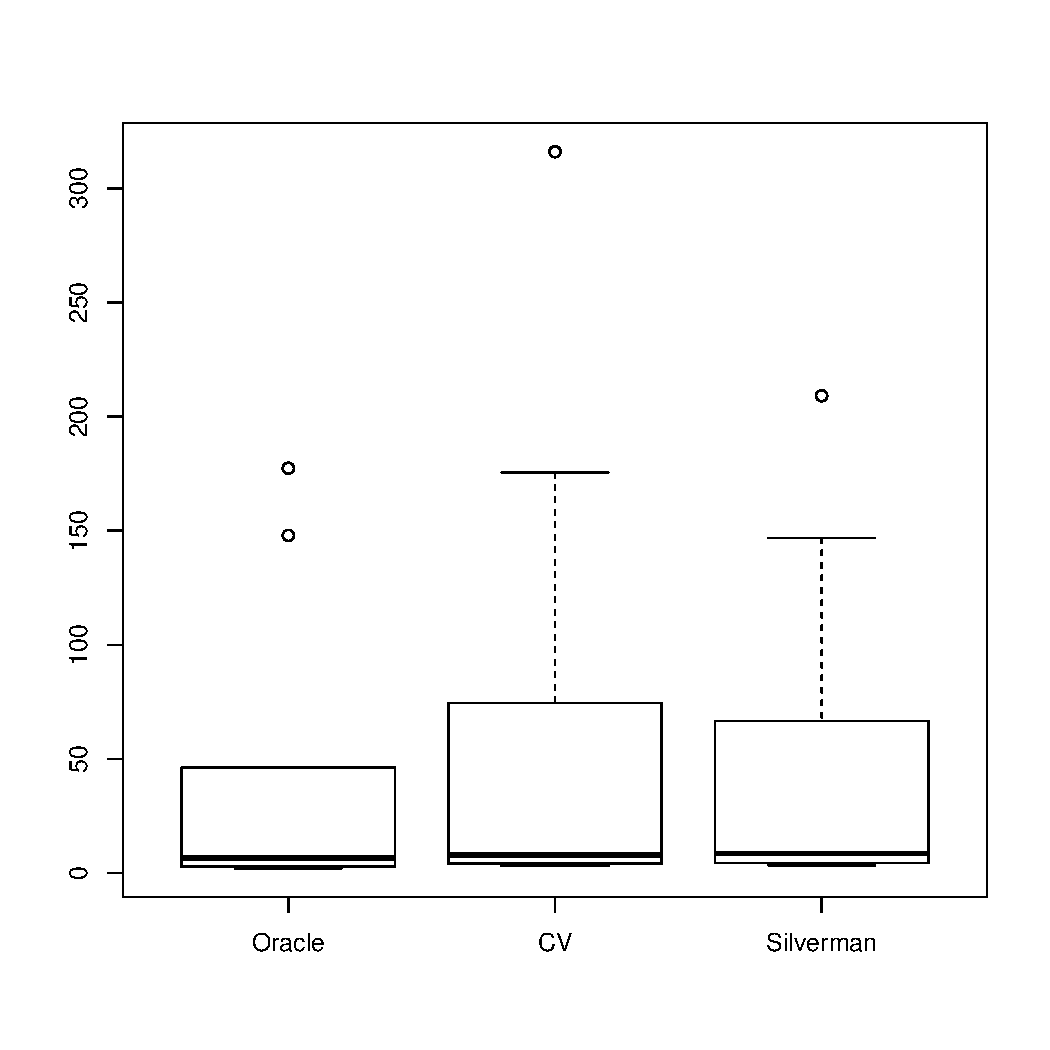
\includegraphics[width=\textwidth]{results/by_overall/normalized-mise-peakpop-boxplot}
        \subcaption{Peaked populations}
        \label{fig:discussion:overall_nmise_boxplot:peak}
    \end{subfigure}
    \caption{Overall distribution of \glsentryname{nmise}}
    \label{fig:discussion:overall_nmise_boxplot}
\end{figure}

As with \gls{nmise}, the \gls{cv} and \gls{silverman} selectors performed similarly to each other.
The 
\begin{figure}[htbp]
    \centering
    \begin{subfigure}[t]{0.45\textwidth}
        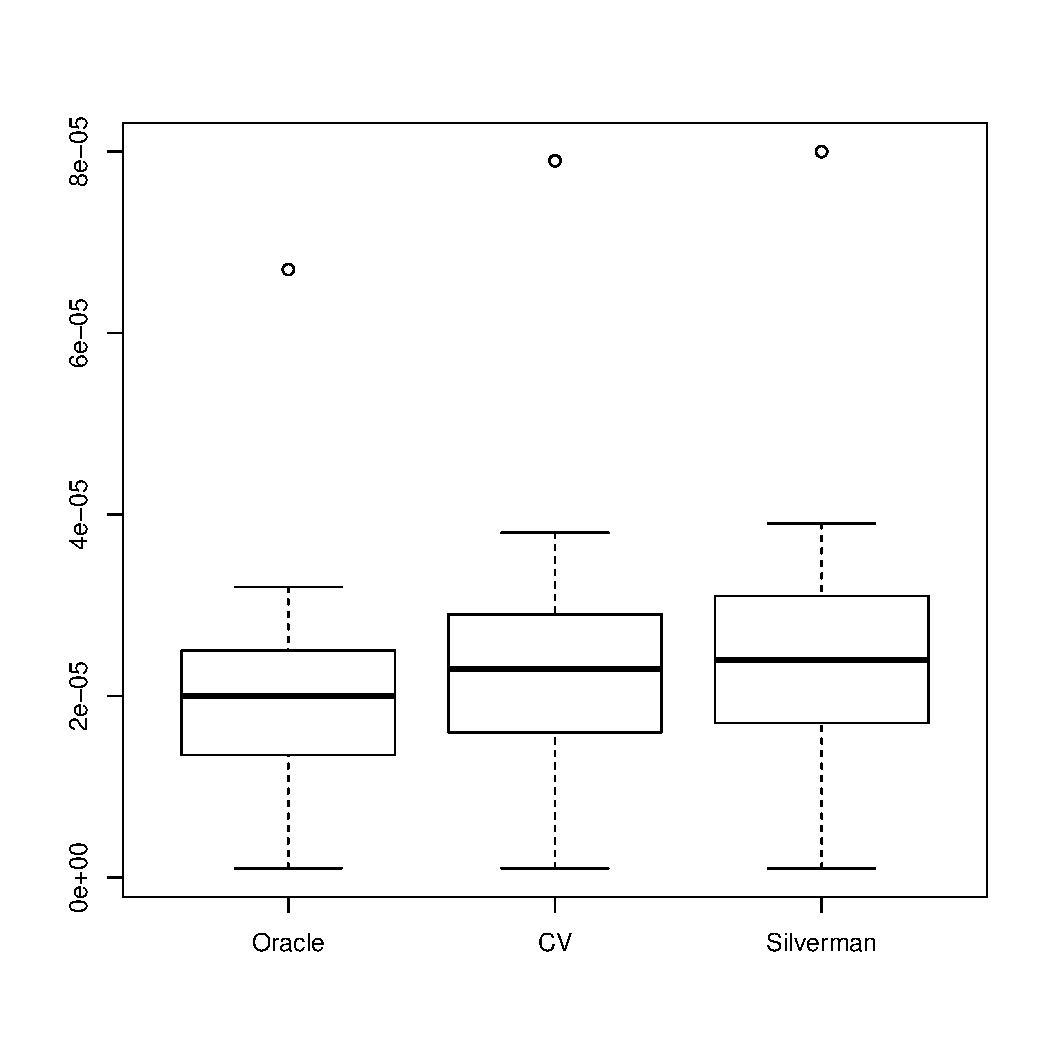
\includegraphics[width=\textwidth]{results/by_overall/normalized-miae-boxplot}
        \subcaption{Uniform populations}
        \label{fig:discussion:overall_nmiae_boxplot:unif}
    \end{subfigure}
    \begin{subfigure}[t]{0.45\textwidth}
        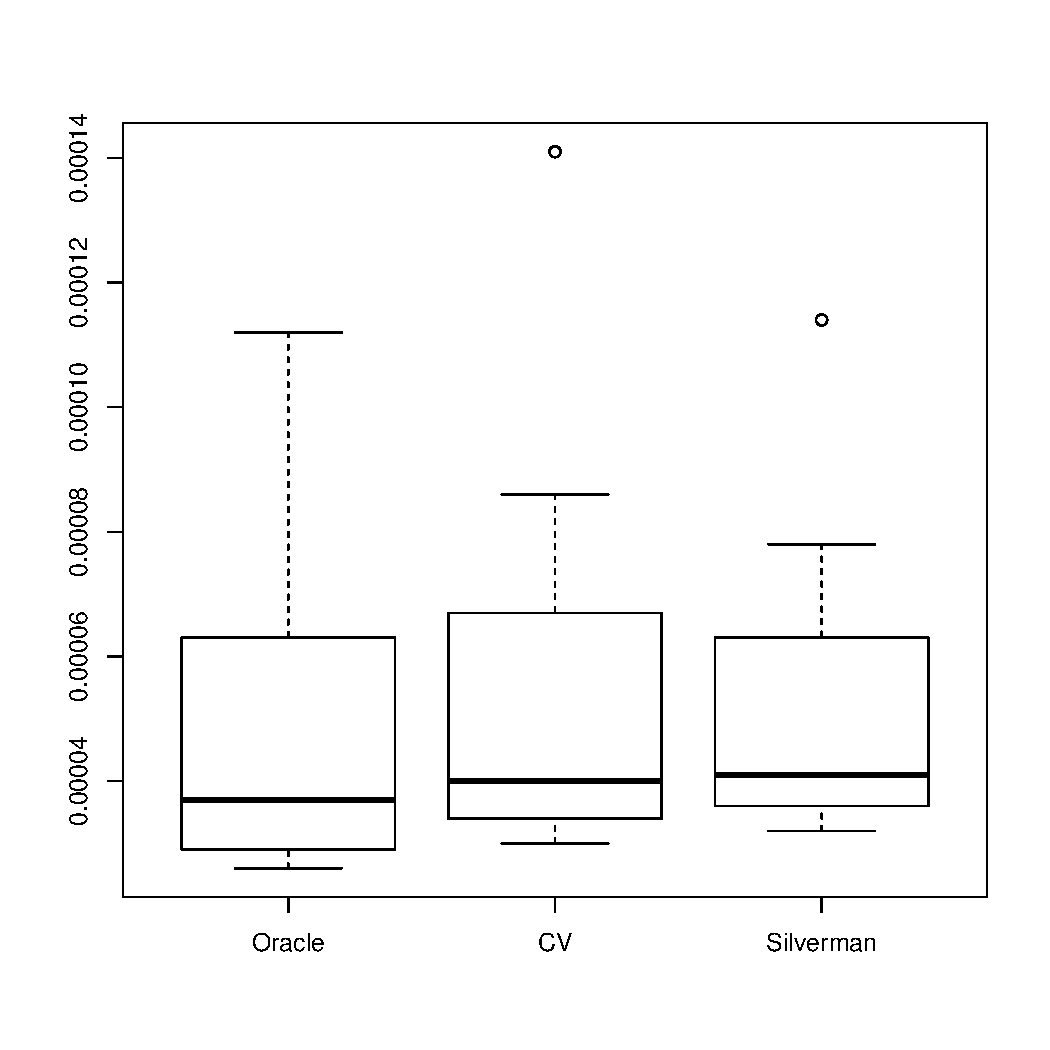
\includegraphics[width=\textwidth]{results/by_overall/normalized-miae-peakpop-boxplot}
        \subcaption{Peaked populations}
        \label{fig:discussion:overall_nmiae_boxplot:peak}
    \end{subfigure}
    \caption{Overall distribution of \glsentryname{nmiae}}
    \label{fig:discussion:overall_nmiae_boxplot}
\end{figure}

\begin{figure}[htbp]
  \centering
  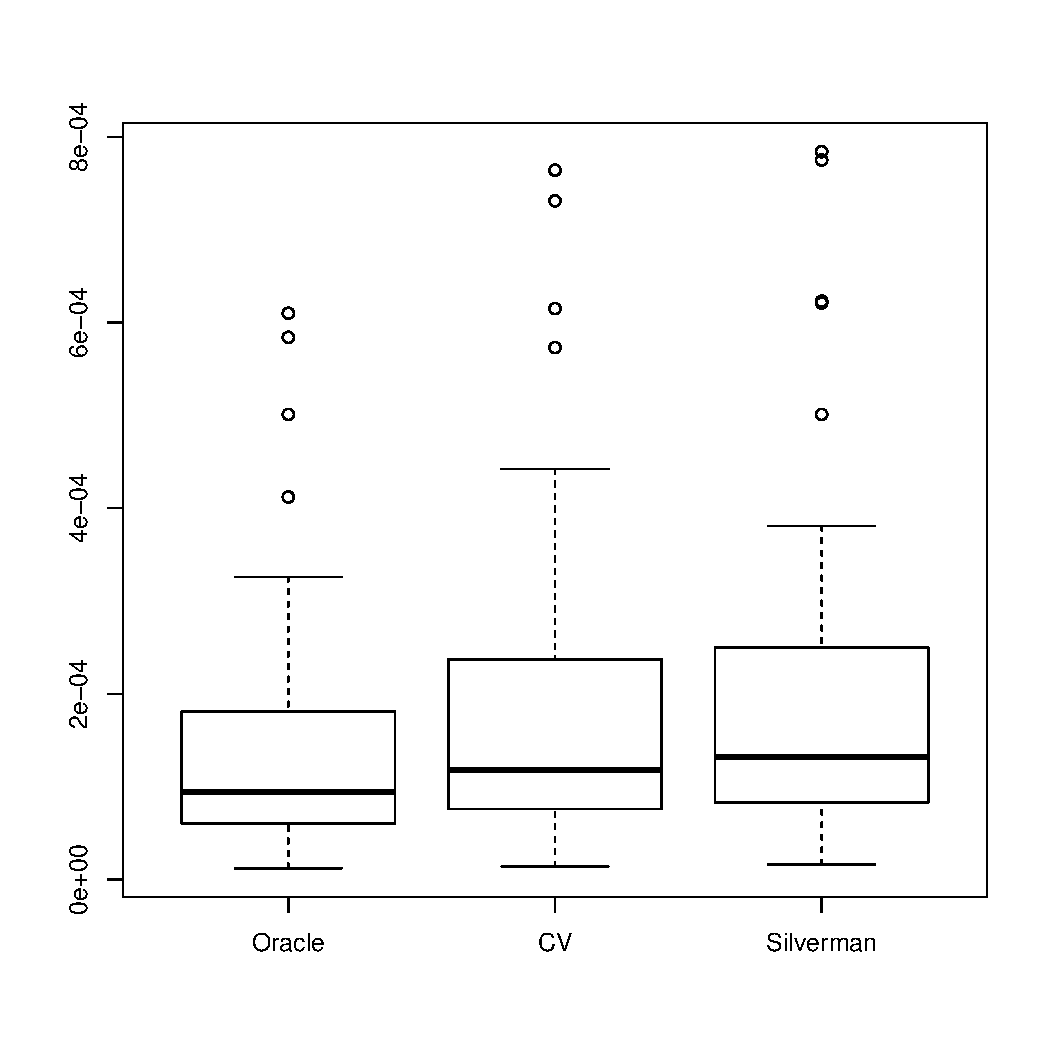
\includegraphics[width=0.45\textwidth]{results/by_overall/normalized-sup-error-boxplot}
  \caption{Overall distribution of \glsentryname{normalized supremum error}}
  \label{fig:discussion:overall_nsup_boxplot}
\end{figure}

\begin{figure}[htbp]
  \centering
  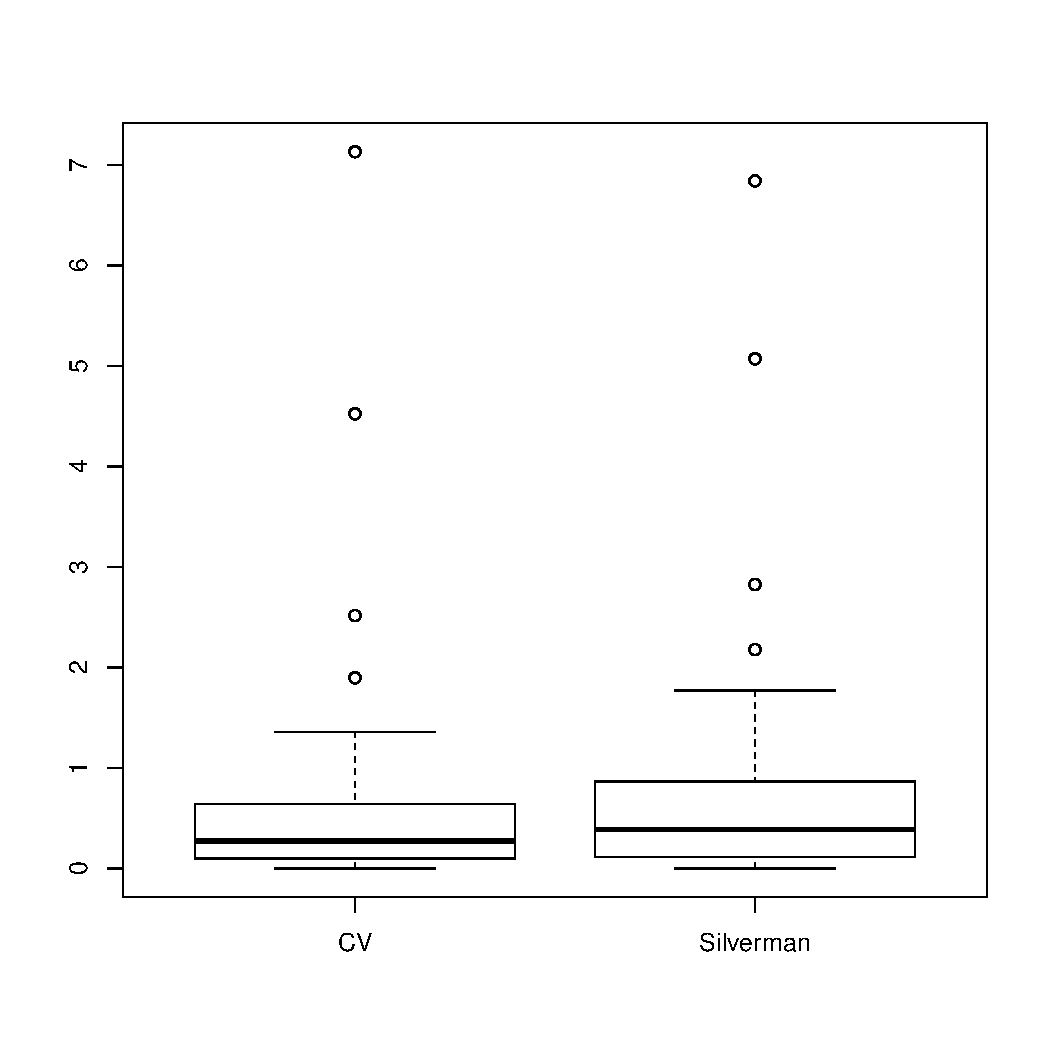
\includegraphics[width=0.45\textwidth]{results/by_overall/normalized-mise-diff-boxplot}
  \caption{Overall distribution of \glsentryname{nmise} difference from the \Glsentryname{oracle}}
  \label{fig:discussion:overall_nmise_diff_boxplot}
\end{figure}


\section{Gradient descent for cross-validation}
\label{sec:discussion:gradient_descent}

We attempted to speed up the cross-validation bandwidth selection by using gradient descent.
We found the gradient descent algorithm often resulted in severe oversmoothing,
as the cross-validation error would decrease slowly as the bandwidth increased.
This required a lot of manual tuning of the learning rate parameter, and so required re-running the experiment several times.
We added \textit{momentum} to our gradient descent implementation but it did not help in every case, and so we changed our strategy to the one described in \Cref{ch:method}.

\section{Accuracy using Silverman}

In \Cref{tab:mean_error_rates:p0.7_100_1.0_1h} we see that the accuracy measure \gls{mise} using the \gls{silverman} rule of thumb is even better than was obtained using the \gls{oracle}.
We tried to run with an additional experiment with 499 monte carlo simulations, and found that in this case the \gls{silverman} rule did not outperform the \gls{oracle}.

